\section{Results and Discussion}

\subsection{Geometry-Preserving Candidate Generation}

Table~\ref{tab:geometry} quantifies candidate generation before any IBO evidence is computed. Direct circular input achieved a class-aware matched rate of 76.87\%. Ordinary unwrapping increased the rate to 79.45\%, whereas extended context alone did not improve the result. Periodic 150-pixel windows achieved 85.77\% and reduced misses from 207 to 88. These results show that the geometry-preserving front end improves candidate availability. They do not, by themselves, demonstrate the contribution of spatial--frequency fusion.

\begin{table}[t]
\caption{Candidate-generation comparison on the 1,124-instance validation set. $C$, $W$, and $M$ denote correct, wrong-class, and missed instances.}
\label{tab:geometry}
\centering
\small
\begin{tabular}{lrrrr}
\toprule
Setting & $C$ & $W$ & $M$ & $C/N$ (\%) \\
\midrule
Circular input & 864 & 53 & 207 & 76.87 \\
Ordinary unwrap & 893 & 63 & 168 & 79.45 \\
Extended context & 884 & 54 & 186 & 78.65 \\
Periodic 150 px & \textbf{964} & 72 & \textbf{88} & \textbf{85.77} \\
\bottomrule
\end{tabular}
\end{table}

\subsection{Industrial Candidate Reliability and Error Trade-off}

Table~\ref{tab:ibo-reliability} reports the completed A0--A5 post-detection evidence ablation. All variants use the same D-FINE candidate groups and class-merging protocol; the operating threshold $t$ is selected separately from each variant's predefined sweep. A0 uses the detector score alone. A1 introduces IBO spatial/group evidence, A2 additionally uses the normal-reference distance, A3 uses local-frequency evidence, A4 combines normal-reference and frequency evidence, and A5 applies restricted gray-versus-collapse confusion-pair correction after A4.

The all-class matched rate changes only slightly from A0 to A4. The principal long-tail effect appears in A5: the focus-tail matched rate rises from 81.56\% to 83.69\%, and gray-weld detection rises from $5/9$ to $8/9$. The explicit collapse-family column exposes the cost of this correction: its matched rate falls from 98.28\% to 94.40\%. Accordingly, all-class $C/N$ decreases by 0.62 points, from 93.67\% to 93.05\%, because a small number of collapse-family instances are reassigned. The result therefore supports the intended interpretation: confusion-pair correction is a targeted tail-recovery mechanism, not an unconditional replacement for the base decision. Figure~\ref{fig:real-corrections} shows two corresponding validation cases: the same local candidate is labeled as gray weld, assigned to the collapse family by D-FINE, and then re-ranked to gray weld by the restricted NORA correction.

\begin{table}[t]
\caption{Completed A0--A5 post-detection evidence ablation on 1,122 class-grouped validation instances. $t$ is selected from the predefined sweep. Tail and collapse entries are $C/N$ (\%); gray-weld entries are $C/W/M$.}
\label{tab:ibo-reliability}
\centering
\scriptsize
\setlength{\tabcolsep}{2.0pt}
\begin{tabular}{clcrrrc}
\toprule
Var. & Evidence added & $t$ & All & Tail & Collapse & Gray \\
\midrule
A0 & D-FINE score & .25 & \textbf{93.67} & 81.56 & \textbf{98.28} & 5/4/0 \\
A1 & + IBO spatial/group & .30 & 93.49 & 80.85 & \textbf{98.28} & 5/4/0 \\
A2 & + normal reference & .35 & 93.49 & 80.85 & \textbf{98.28} & 5/4/0 \\
A3 & + local frequency & .10 & 93.58 & 81.56 & \textbf{98.28} & 5/4/0 \\
A4 & + normal reference + frequency & .15 & 93.58 & 81.56 & \textbf{98.28} & 5/4/0 \\
A5 & + restricted confusion correction & .15 & 93.05 & \textbf{83.69} & 94.40 & \textbf{8/1/0} \\
\bottomrule
\end{tabular}
\end{table}
\begin{table*}[!t]
\caption{Primary in-house comparison under the 1,122-instance class-grouped audit. All methods use no-stretch periodic 150-pixel seam strips. D-FINE-S, SimLTD-style, and NORA share the D-FINE-S detector, whereas ROG uses its Faster R-CNN implementation. FRACAL$^{\dagger}$ is a budget-matched calibration of a separately frozen D-FINE-S candidate generator at $t=.056$, rather than a matched-decision detector run; its source audit does not contain the identical focus-tail aggregate, hence ``--''. $C/W/M$ reports correct, wrong-class, and missed instances. Tail and collapse values are matched rate $C/N$ (\%); gray-weld is $(C/W/M)$.}
\label{tab:inhouse-comparison}
\centering
\small
\setlength{\tabcolsep}{4.0pt}
\begin{tabular}{lllrrrrr}
\toprule
Method & Decision setting & Input & $C/W/M$ & All $C/N$ & Tail $C/N$ & Gray & Collapse $C/N$ \\
\midrule
D-FINE-S & detector score, $t=.25$ & periodic 150-px strip & 1051/44/27 & \textbf{93.67} & 81.56 & 5/4/0 & \textbf{98.28} \\
SimLTD-style & 20/6/6 head--tail--joint schedule, $t=.25$ & periodic 150-px strip & 1028/57/37 & 91.62 & 80.85 & 0/8/1 & 91.81 \\
ROG & Faster R-CNN R50FPN transfer, $t=.25$ & periodic 150-px strip & 948/71/103 & 84.49 & 74.47 & 0/1/8 & 83.62 \\
FRACAL$^{\dagger}$ & budget-matched calibration, $t=.056$ & periodic 150-px strip & 931/147/44 & 82.98 & -- & 3/6/0 & 93.53 \\
NORA (A4) & IBO + normal reference + frequency, $t=.15$ & periodic 150-px strip & 1050/45/27 & 93.58 & 81.56 & 5/4/0 & \textbf{98.28} \\
NORA (A5) & A4 + restricted confusion correction, $t=.15$ & periodic 150-px strip & 1044/51/27 & 93.05 & \textbf{83.69} & \textbf{8/1/0} & 94.40 \\
\bottomrule
\end{tabular}
\end{table*}
\begin{figure*}[t]
\centering
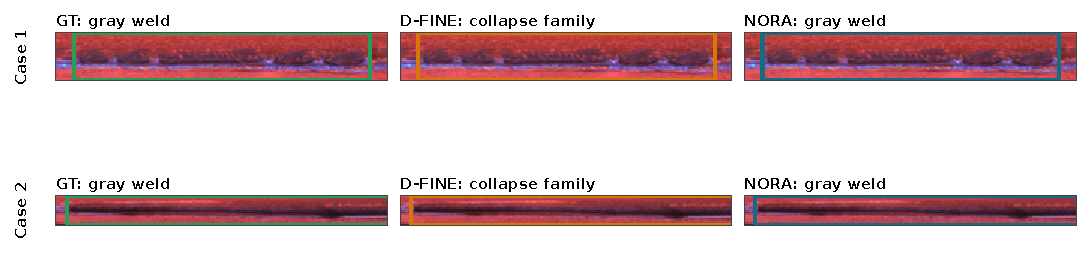
\includegraphics[width=\textwidth]{figures/fig2_real_nora_corrections.pdf}
\caption{Two real validation cases corrected by the restricted gray-weld versus collapse-family module. Each row shows the same no-stretch weld-strip crop. D-FINE assigns the candidate to the collapse family, whereas NORA re-ranks it as gray weld, matching the annotation. These examples visualize the targeted tail recovery quantified in Table~\ref{tab:ibo-reliability}; they do not imply that every collapse-family prediction should be changed.}
\label{fig:real-corrections}
\end{figure*}
\subsection{LVIS Pilot: Transfer of Candidate Reliability}
\label{sec:lvis-results}

The LVIS pilot evaluates normal-reference evidence outside annular-weld geometry. On 33,006 validation candidates, the reliability model achieved AUROC $=0.6890$, AUPR $=0.5275$, and Brier score $=0.2511$. Table~\ref{tab:lvispilot} reports the official-LVIS API results; candidate recovery is reported in the accompanying thresholded-projection audit. Relative to the D-FINE score threshold of 0.40, reliability threshold 0.15 retained more candidates, increased correctly covered instances by 1,945, and reduced misses by 3,990. It also increased wrong-class instances by 2,045. The 9.31-point gain in $C/N$ is therefore a recall-oriented candidate-recovery result, not a free improvement in final classification.

\begin{table*}[!t]
\caption{LVIS pilot method comparison under the official LVIS API. AP, AP50, AP75, APr, APc, and APf are percentage metrics. All methods use the same 10k/2k pilot split and 640-pixel no-stretch input. D-FINE-S and NORA share the frozen 100-epoch D-FINE-S candidate generator; FRACAL recalibrates its outputs with an equal per-image prediction budget; ROG is an independently trained Faster R-CNN R50FPN transfer model run for 32 epochs; and SimLTD uses its public codebase with a 20/6/6 fast-pilot schedule, not the full official schedule. Candidate-level $C/N$ is discussed separately because it uses a thresholded projection audit rather than the full prediction ranking.}
\label{tab:lvispilot}
\centering
\scriptsize
\setlength{\tabcolsep}{3.2pt}
\begin{tabular}{lllrrrrrr}
\toprule
Method & Learning setting & Input & AP & AP50 & AP75 & APr & APc & APf \\
\midrule
D-FINE-S & raw candidate ranking & 640, no stretch & 8.008 & 11.869 & 8.218 & 0 & 2.096 & 12.165 \\
FRACAL & inference-only, budget-matched recalibration & 640, no stretch & 8.457 & 12.583 & 8.588 & .223 & 2.584 & 12.612 \\
ROG & Faster R-CNN R50FPN transfer, epoch 32 & 640, no stretch & 10.800 & 21.200 & 9.800 & 2.400 & 9.400 & 12.300 \\
SimLTD & public codebase, 20/6/6 fast pilot & 640, no stretch & \textbf{12.700} & \textbf{20.600} & \textbf{12.900} & \textbf{6.600} & \textbf{11.300} & \textbf{14.100} \\
NORA & IBO reliability, $t=.15$ & 640, no stretch & 8.008 & 11.869 & 8.218 & 0 & 2.096 & 12.165 \\
NORA & reliability + restricted correction & 640, no stretch & 8.008 & 11.869 & 8.218 & 0 & 2.096 & 12.165 \\
\bottomrule
\end{tabular}
\end{table*}

The local query corrector used 15 confusion-cluster models derived from 30 training-only confusion edges. At probability/margin gates $(0.55,0.15)$, it re-ranked 2 of 33,006 validation candidates. At $(0.65,0.20)$, it re-ranked none. The corresponding $(C,W,M)$ summaries were unchanged. The restriction avoids broad label-space changes, but it is too conservative to demonstrate an aggregate gain in this pilot.

For benchmark alignment, we additionally exported the frozen candidate outputs to the official LVIS API. The raw candidate set obtained AP $=8.008\%$, AP50 $=11.869\%$, AP75 $=8.218\%$, APr $=0$, APc $=2.096\%$, and APf $=12.165\%$. FRACAL's budget-matched recalibration raised AP to $8.457\%$. The completed SimLTD fast pilot reached AP $=12.700\%$, AP50 $=20.600\%$, AP75 $=12.900\%$, APr $=6.600\%$, APc $=11.300\%$, and APf $=14.100\%$. This SimLTD row uses the public codebase and the official LVIS evaluator, but its shortened 20/6/6 schedule is not a full official-schedule reproduction. Reliability filtering and the restricted corrector changed NORA's AP by less than $0.001$ percentage points. Thus, the present pilot supports candidate-level recovery but does \emph{not} demonstrate an official LVIS AP gain; this distinction is maintained by reporting official AP separately from the candidate-projection audit.

\subsection{Scope of the Fusion Claim}

The completed industrial and LVIS studies support three narrower findings. Cyclic geometry improves candidate availability. Normal-reference evidence can retain low-score candidates. Conservative local correction does not produce measurable global degradation in this pilot. The studies do not yet establish that the learned query-level fusion in Section~\ref{sec:reliability-fusion} outperforms fixed spatial--frequency concatenation. That claim requires the B0--B6 comparison specified in Section~3, particularly B3 (fixed fusion), B4 (normal-reference conditioning), and B5 (reliability plus disagreement). Stating this boundary prevents candidate-stage improvements from being interpreted as an end-to-end detector gain.
